\documentclass[14pt,aspectratio=1610]{beamer}

\usepackage[brazil]{babel}
\usepackage[utf8]{inputenc}
%\UseRawInputEncoding
\usepackage[T1]{fontenc}
%\usepackage{Sweave}
\usepackage{animate}
\usepackage{amsbsy}
\usepackage{amsfonts}
\usepackage{amsmath}
\usepackage{amssymb}
\usepackage{amsthm}
\usepackage[toc,page,title,titletoc]{appendix}
%\usepackage[fixlanguage]{babelbib}
%\usepackage[pdftex]{color}
\usepackage{dsfont}
\usepackage{esvect}
\usepackage[labelfont=bf]{caption}
\usepackage{subcaption}
\usepackage{float}
\usepackage[Glenn]{fncychap}%Sonny %Conny %Lenny %Glenn %Renje %Bjarne %Bjornstrup
%\usepackage{geometry, calc, color, setspace}%
%\geometry{a4paper, headsep=1.0cm, footskip=1cm, lmargin=3cm, rmargin=2cm, tmargin=3cm, bmargin=2cm}
\usepackage{graphicx}
\usepackage{indentfirst}%Para indentar os parágrafos automáticamente
\usepackage{lipsum}
\usepackage{longtable}
\usepackage{mathtools}
\usepackage{listings}%Inserir codigo do R no latex
%\usepackage{slashbox}
\usepackage{multirow}
\usepackage{multicol}
\usepackage{csquotes}
\usepackage[maxcitenames=2,terseinits=true,natbib=true, style=authoryear, maxbibnames=99]{biblatex}
\addbibresource{../Referencias/Referencias.bib}
\usepackage[figuresright]{rotating}
\usepackage{spalign}
%\usepackage{pgfpages}
\usepackage{pgfplots}
\pgfplotsset{compat=1.18}
\usepackage{tikz}
\usepackage{color, colortbl}
\usepackage{ragged2e}%para justificar o texto dentro de algum ambiente
\definecolor{Gray}{gray}{0.9}
\definecolor{LightCyan}{rgb}{0.88,1,1}
\definecolor{Lightblue}{RGB}{50, 149, 168}
%\usepackage{grffile}

\usepackage[all]{xy}



%\usetheme{Madrid}
%\usecolortheme[RGB={193,0,0}]{structure}
\usetheme{metropolis}
\definecolor{mycolor}{RGB}{34, 45, 50}
\setbeamercolor{structure}{fg=mycolor}
\usepackage{mathpazo} % Fonte elegante para matemática
\usepackage{helvet} % Fonte sans-serif para texto
\renewcommand{\familydefault}{\sfdefault} % Definir fonte padrão como sans-serif

%\setbeamertemplate{footline}[frame number]
%\setbeamertemplate{footline}[text line]{%
	%  \parbox{\linewidth}{\vspace*{-8pt}\hfill\date{}\hfill\insertshortauthor\hfill\insertpagenumber}}
\beamertemplatenavigationsymbolsempty
\renewcommand{\vec}[1]{\mbox{\boldmath$#1$}}
\newtheorem{Teorema}{Teorema}
\newtheorem{Proposicao}{Proposição}
\newtheorem{Definicao}{Definição}
\newtheorem{Corolario}{Corolário}
\newtheorem{Demonstracao}{Demonstração}
\newcommand{\bx}{\ensuremath{\bar{x}}}
\newcommand{\Ho}{\ensuremath{H_{0}}}
\newcommand{\Hi}{\ensuremath{H_{1}}}
\everymath{\displaystyle}

\apptocmd{\frame}{}{\justifying}{} % Allow optional arguments after frame.

\title{Estatística I}
\author{Prof. Fernando de Souza Bastos \texorpdfstring{\\ fernando.bastos@ufv.br}{}}
\institute{Departamento de Estatística \texorpdfstring{\\ Universidade Federal de Viçosa}{}\texorpdfstring{\\ Campus UFV - Viçosa}{}}
\date{}
\newcommand\mytext{Aula 19}
\newcommand\mytextt{Fernando de Souza Bastos}
\newcommand\mytexttt{\url{https://ufvest.github.io/}}

\makeatletter
\setbeamertemplate{footline}
{
	\leavevmode%
	\hbox{%
		\begin{beamercolorbox}[wd=.3\paperwidth,ht=2.25ex,dp=1ex,center]{author in head/foot}%
			\usebeamerfont{author in head/foot}\mytext
		\end{beamercolorbox}%
		\begin{beamercolorbox}[wd=.3\paperwidth,ht=2.25ex,dp=1ex,center]{title in head/foot}%
			\usebeamerfont{title in head/foot}\mytextt
		\end{beamercolorbox}%
		\begin{beamercolorbox}[wd=.35\paperwidth,ht=2.25ex,dp=1ex,right]{site in head/foot}%
			\usebeamerfont{site in head/foot}\mytexttt\hspace*{2em}
			\insertframenumber{} / \inserttotalframenumber\hspace*{2ex} 
	\end{beamercolorbox}}%
	\vskip0pt%
}
\makeatother

\providecommand{\arcsin}{} \renewcommand{\arcsin}{\hspace{2pt}\textrm{arcsen}}
\providecommand{\sin}{} \renewcommand{\sin}{\hspace{2pt}\textrm{sen}}
%\newtheorem{Teorema}{Teorema}
%\newtheorem{Proposicao}{Proposição}
%\newtheorem{Definicao}{Definição}
%\newtheorem{Corolario}{Corolário}
%\newtheorem{Demonstracao}{Demonstração}

\titlegraphic{\hspace*{8cm}\href{https://fsbmat-ufv.github.io/}{
\includegraphics[width=2cm]{figs/mylogo.png}}
}


\usepackage{hyperref,bookmark}
\hypersetup{
	colorlinks=true,
	linkcolor=blue,
	citecolor=red,
	filecolor=blue,
	urlcolor=blue,
}

% Layout da pagina
\hypersetup{pdfpagelayout=SinglePage}
\begin{document}
	%\input{Aula21-concordance}
	
	\frame{\titlepage}
	
	\begin{frame}{}
		\frametitle{\bf Sumário}
		\tableofcontents
	\end{frame}
	
\section{Introdução}

\begin{frame}{Por que não confiar só na média?}
	
	\begin{block}{}
		\justifying
		
		Imagine que você está com muita fome e abre o aplicativo de delivery. A informação aparece assim:
		
		\begin{center}
			\textbf{"O tempo médio de entrega é de 30 minutos."}
		\end{center}
		
		Você pensa:
		
		\textit{"Perfeito! Em meia horinha eu tô comendo!"}
		
	\end{block}
	
\end{frame}

\begin{frame}{Por que não confiar só na média?}
	
	\begin{block}{}
		\justifying
		
		Mas... será que é tão simples assim?
		
		Pense nos dados que o aplicativo usa para calcular essa média:
		
		\begin{itemize}
			\item Algumas entregas foram muito rápidas (15, 20 minutos).
			\item Outras demoraram bastante (60, 70, até 90 minutos).
		\end{itemize}
		
		A \textbf{média} de 30 minutos parece bonita... mas esconde toda essa variabilidade!
		
	\end{block}
	
\end{frame}

\begin{frame}{A verdade por trás da média}
	\small
	\begin{block}{}
		\justifying
		
		Se o aplicativo dissesse:
		
		\begin{center}
			\textbf{"Com 95\% de confiança, seu pedido chegará entre 20 minutos e 1 hora e 10 minutos."}
		\end{center}
		
		Agora sim, você entende o jogo!
		
		Isso significa que:
		
		\begin{itemize}
			\item É possível que chegue rápido (20 min).
			\item Mas também existe uma chance real de demorar mais de uma hora.
		\end{itemize}
		
		\textbf{Percebe a diferença?}
		
		\begin{center}
			\textit{"A média é uma informação solitária. O intervalo de confiança é uma informação honesta."}
		\end{center}
		
	\end{block}
	
\end{frame}

\begin{frame}{}
	
	\begin{block}{}
		\justifying
		
		\begin{center}
			\textit{"A média é uma informação solitária. O intervalo de confiança é uma informação honesta."}
		\end{center}
		\pause
		\begin{center}
			\textit{Confiar só na média é como dirigir olhando apenas pelo retrovisor... Parece informação, mas não te mostra o que vem pela frente.}
		\end{center}
		
	\end{block}
\end{frame}	
	
	\begin{frame}{Dois tipos de estimativas}
		
		\begin{block}{Estimativa Pontual}
			\justifying
			É quando usamos um único número, calculado a partir da amostra, para estimar um parâmetro populacional.
			
			\vspace{0.2cm}
			\textbf{Exemplos:}
			\begin{itemize}
				\item Média amostral (\( \bar{x} \)) para estimar a média populacional (\( \mu \)).
				\item Proporção amostral (\( \hat{p} \)) para estimar a proporção populacional (\( p \)).
			\end{itemize}
			
			\textbf{Limitação:} Fornece apenas um valor. Não diz nada sobre a incerteza ou confiabilidade desse valor.
		\end{block}
		
	\end{frame}
	
	\begin{frame}{Dois tipos de estimativas}
			
		\begin{block}{Estimativa Intervalar (Intervalo de Confiança)}
			\justifying
			Em vez de fornecer um único número, fornece um \textbf{intervalo de valores plausíveis} para o parâmetro populacional.
			
			\vspace{0.2cm}
			\textbf{Exemplo:}
			\begin{center}
				\textit{"Com 95\% de confiança, a média populacional está entre 25 e 35."}
			\end{center}
			
			\textbf{Vantagem:} Expressa não só a estimativa, mas também a incerteza associada a ela.
		\end{block}
		
	\end{frame}
	
	\begin{frame}{Por que precisamos de um intervalo de confiança?}
		\small
		\vspace{-0.3cm}
		\begin{block}{}
			\justifying
			
			Todo estimador (como a média amostral) é uma \textbf{variável aleatória}.
				\vspace{-0.3cm}
			\begin{itemize}
				\item Se coletarmos outra amostra, vamos obter outro valor.
				\item A cada amostra possível, temos uma média diferente.
			\end{itemize}
				\vspace{-0.3cm}
			Por isso, o estimador possui uma \textbf{distribuição de probabilidade}, chamada de \textbf{distribuição amostral}.
			
			\textbf{E é exatamente a partir dessa distribuição que construímos o intervalo de confiança.}

			
			O intervalo de confiança nos permite afirmar algo do tipo:
			
			\begin{center}
				\textit{"Se eu repetir esse processo muitas vezes, 95\% dos intervalos conterão o verdadeiro valor do parâmetro."}
			\end{center}
			
		\end{block}
		
	\end{frame}
	

\begin{frame}{Visualizando a incerteza}
	\vspace{-0.3cm}
	\begin{block}{}
		\centering
		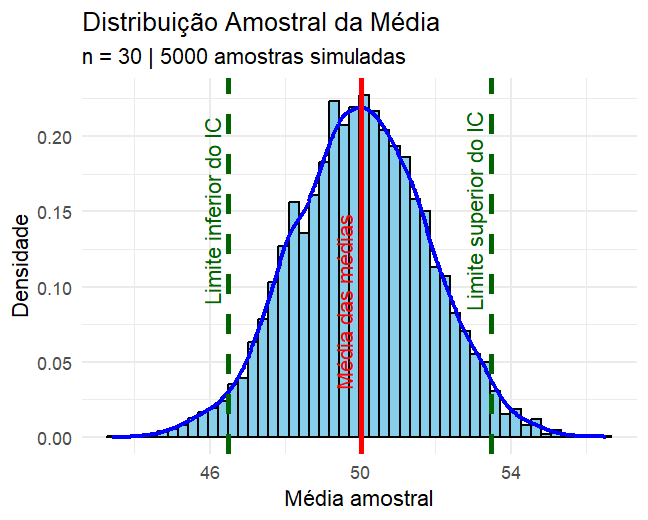
\includegraphics[width=0.7\linewidth]{figs/Intervalo.png}
	\end{block}
	
\end{frame}

	
\section{Intervalos de Confiança para a Média: $\sigma$ conhecido}

\begin{frame}{Suposições Necessárias}
	\begin{block}{}
		\justifying
		Para construirmos um intervalo de confiança para a média (com $\sigma$ conhecido), precisamos garantir:
		\begin{itemize}
			\item A amostra é uma \textbf{amostra aleatória simples (AAS)}.
			\item O desvio padrão da população ($\sigma$) é conhecido.
			\item E uma das seguintes condições:
			\begin{itemize}
				\item A população tem distribuição normal;
				\item ou o tamanho da amostra é suficientemente grande ($n > 30$).
			\end{itemize}
		\end{itemize}
	\end{block}
\end{frame}

\begin{frame}{Erro Amostral: Sempre Existe!}
	\small
	\begin{block}{}
		\justifying
		Ao coletar uma amostra, a média amostral ($\bar{X}$) dificilmente será exatamente igual à média populacional ($\mu$).
		
		\textbf{Essa diferença é chamada de erro amostral:}
		
		\[
		e = \bar{X} - \mu \quad \Leftrightarrow \quad \bar{X} = \mu + e
		\]
		
		Sabemos que a média amostral segue uma distribuição:
		
		\[
		\bar{X} \sim \text{N}\left(\mu, \frac{\sigma^2}{n}\right)
		\]
		
		Ou seja, as médias amostrais \textbf{variam} de amostra para amostra!
	\end{block}
\end{frame}

\begin{frame}{O que é a Margem de Erro?}
	\small
	\vspace{-0.3cm}
	\begin{block}{}
		\justifying
		Se padronizarmos a média amostral, obtemos:
		
		\[
		Z = \frac{\bar{X} - \mu}{\sigma / \sqrt{n}} \sim \text{N}(0,1)
		\]
		
		\textbf{Z responde:} Quantos desvios padrão minha média amostral está distante da média populacional.
		
		A \textbf{margem de erro} ($e$) representa o erro máximo aceitável, dentro de um grau de confiança ($\gamma$):
		
		\[
		e = z_{\gamma/2} \cdot \frac{\sigma}{\sqrt{n}}
		\]
		
		Onde $z_{\gamma/2}$ é o \textbf{valor crítico da normal padrão}.
	\end{block}
\end{frame}

\begin{frame}{Construindo o Intervalo de Confiança}
	\begin{block}{Raciocínio}
		\justifying
		Queremos capturar o valor de $\mu$ dentro de um intervalo simétrico ao redor da média amostral $\bar{x}$.
		\vspace{-0.3cm}
		\[
		P\left( -z_{\gamma/2} < Z < z_{\gamma/2} \right) = \gamma
		\]
			\vspace{-0.3cm}
		Substituindo $Z$ pela padronização da média:
		
		\[
		P\left( \bar{x} - z_{\gamma/2} \cdot \frac{\sigma}{\sqrt{n}} < \mu < \bar{x} + z_{\gamma/2} \cdot \frac{\sigma}{\sqrt{n}} \right) = \gamma
		\]
		
		\textbf{Pronto!} Este é o intervalo de confiança para $\mu$ com confiança $\gamma$.
	\end{block}
\end{frame}

\begin{frame}{Valor Crítico $z_{\gamma/2}$}
	\begin{block}{}
		\justifying
		O valor $z_{\gamma/2}$ é o ponto da distribuição normal padrão que deixa uma área de $\gamma/2$ em cada cauda.
		
		Por exemplo, para $\gamma = 0,95$:
		\begin{itemize}
			\item A área central é 95\%.
			\item Sobra 5\% para as caudas → 2,5\% em cada lado.
			\item Buscamos na tabela da normal padrão a área acumulada até 0,975.
			\item Resultado: $z_{0,025} = 1,96$.
		\end{itemize}
	\end{block}
	
	\centering
	%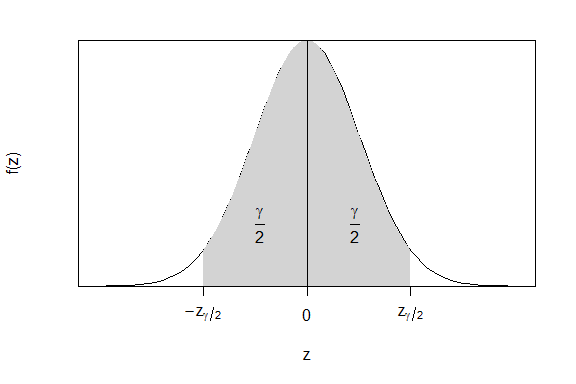
\includegraphics[width=0.75\linewidth]{figs/IC2.png}
	
	\small\textit{A área central corresponde ao nível de confiança $\gamma$.}
\end{frame}

\begin{frame}{Fórmula do Intervalo de Confiança}
	\begin{block}{}
		O intervalo de confiança para $\mu$, com nível de confiança $\gamma$, é dado por:
		
		\[
		\left[
		\bar{X} - z_{\gamma/2} \cdot \frac{\sigma}{\sqrt{n}} \; ; \;
		\bar{X} + z_{\gamma/2} \cdot \frac{\sigma}{\sqrt{n}}
		\right]
		\]
		
		\textbf{Interpretação:} Uma faixa de valores plausíveis para a média populacional, considerando a variabilidade natural das amostras.
	\end{block}
\end{frame}

\begin{frame}{Passos para construir o Intervalo de Confiança}
	\begin{enumerate}
		\item Verificar as suposições:
		\begin{itemize}
			\item AAS
			\item $\sigma$ conhecido
			\item População normal ou $n > 30$
		\end{itemize}
		\item Escolher o nível de confiança $\gamma$ e determinar $z_{\gamma/2}$.
		\item Calcular a margem de erro:
		\[
		e = z_{\gamma/2} \cdot \frac{\sigma}{\sqrt{n}}
		\]
		\item Construir o intervalo:
		\[
		\bar{X} \pm e
		\]
	\end{enumerate}
\end{frame}

\begin{frame}{Interpretação do Intervalo de Confiança}
	\begin{block}{Atenção: O que significa $\gamma$?}
		\justifying
		- O \textbf{parâmetro} ($\mu$) é fixo.  
		- O que varia é o \textbf{intervalo}, porque ele depende da amostra.  
		
		Se construirmos 100 intervalos de confiança de 95\%, usando 100 amostras diferentes, \textbf{esperamos que 95 deles contenham $\mu$}, e 5 não contenham.
		
		\textbf{Importante:} \textit{Não dizemos que "a probabilidade de $\mu$ estar no intervalo é 95\%". $\mu$ não é aleatório. O que é aleatório é o intervalo.}
	\end{block}
\end{frame}

	
	\begin{frame}{}
		\begin{block}{}
			\justifying
			\begin{figure}
				\centering
				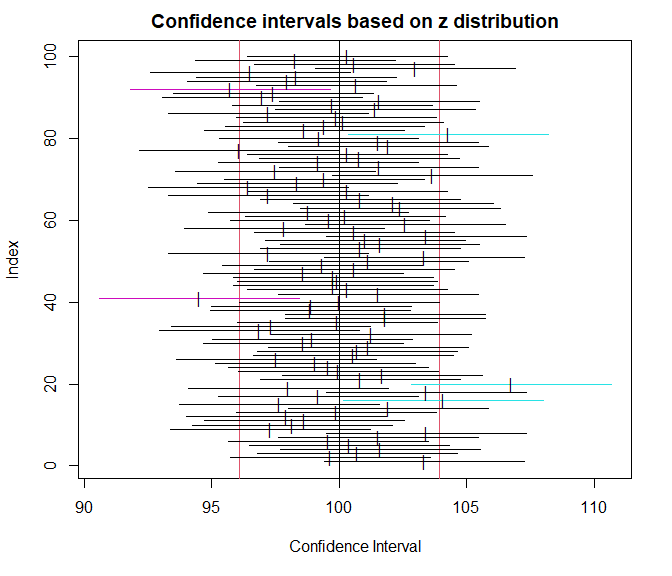
\includegraphics[scale=0.6]{figs/IC3.png}
			\end{figure}
		\end{block}
	\end{frame}
	
	\begin{frame}{Exemplo}
		\begin{block}{}
			\justifying
			Uma empresa de marketing deseja estimar quanto tempo, em m\'edia, as pessoas passam no WhatsApp por semana.
			
			Eles selecionaram, aleatoriamente, uma amostra de 25 pessoas. O tempo m\'edio de uso foi de \textbf{22,4 horas por semana} \textendash{} isso mesmo, quase um emprego de meio per\'iodo s\'o no zap!
			
			Com base em estudos anteriores, eles assumem que o desvio padr\~ao populacional \'e $\sigma = 5,2$ horas e que o tempo de uso tem distribui\c{c}\~ao normal.
			
			Construa um intervalo de confian\c{c}a de 95\% para a m\'edia populacional $\mu$.
		\end{block}
		
	\end{frame}
	
	\begin{frame}{Exemplo}
	
		\begin{block}{Solu\c{c}\~ao}
			\[
			\bar{X} = 22,4, \quad n = 25, \quad \sigma = 5,2
			\]
			\[
			z_{0,025} = 1,96
			\]
			\[
			e = 1,96 \cdot \frac{5,2}{\sqrt{25}} = 2,038
			\]
			\[
			IC = \left[22,4 - 2,038 \; ; \; 22,4 + 2,038\right]
			\]
			\[
			(20,362 \leq \mu \leq 24,438)
			\]
			\textbf{Interpreta\c{c}\~ao:} Com 95\% de confian\c{c}a, o tempo m\'edio que as pessoas passam no WhatsApp por semana est\'a entre aproximadamente \textbf{20,4 e 24,4 horas}.
		\end{block}
	\end{frame}
	
	
	
%%%%%%%%%%%%%%%%%%%%%%%%%%%%%%%%%%%%%%%%%%%%%%%%%%%%%%%%%%%%%%%%%%%%
\section{Intervalos de Confiança para a Média: $\sigma$ desconhecido}

\begin{frame}{Quando $\sigma$ é Desconhecido}
	\small
	\begin{block}{Estimativa da Variância Amostral}
		\justifying
		Na maioria das situações práticas, não sabemos o verdadeiro valor do desvio padrão populacional ($\sigma$). Se $\sigma$ é desconhecido, ele precisa ser estimado a partir da amostra.
		
		Sendo $(X_1, \ldots, X_n)$ uma amostra aleatória de uma variável aleatória $X \sim \text{N}(\mu, \sigma^2)$, o estimador da variância populacional é a variância amostral:
		
		\[
		S^2 = \frac{1}{n-1} \sum_{i=1}^n (X_i - \bar{X})^2
		\]
		
		Esse estimador é \textbf{não viciado} e \textbf{consistente} para $\sigma^2$.
	\end{block}
\end{frame}

\begin{frame}{A Distribuição $t$ de Student}
	\small
	\begin{block}{}
		\justifying
		Quando substituímos $\sigma$ pela estimativa $S$, a variável padronizada passa a ser:
		
		\[
		T = \frac{\bar{X} - \mu}{S / \sqrt{n}}
		\]
		
		Essa variável não segue mais a distribuição normal. Ela segue uma \textbf{distribuição $t$ de Student} com \textbf{$n-1$ graus de liberdade}:
		
		\[
		T \sim t(n-1)
		\]
		
		A distribuição $t$ é mais "espalhada" que a normal, pois leva em conta a incerteza adicional de estimar $\sigma$.
	\end{block}
\end{frame}

\begin{frame}{Valores Críticos da Distribuição $t$}
	\begin{block}{}
		\justifying
		Para determinar o valor crítico $t_{\gamma/2}$, usamos:
		\begin{itemize}
			\item O nível de confiança ($\gamma$);
			\item O número de graus de liberdade ($gl = n - 1$).
		\end{itemize}
		
		Exemplo:
		\begin{itemize}
			\item $\gamma = 95\%$ e $n = 7 \Rightarrow gl = 6$
			\item Buscamos na tabela $t$ a linha dos $gl = 6$ e a coluna correspondente a $5\%$ (2,5\% em cada cauda)
			\item Encontramos: $t_{0,025} = 2,447$
		\end{itemize}
	\end{block}
\end{frame}

\begin{frame}{Distribuição $t$ de Student}
	\centering
	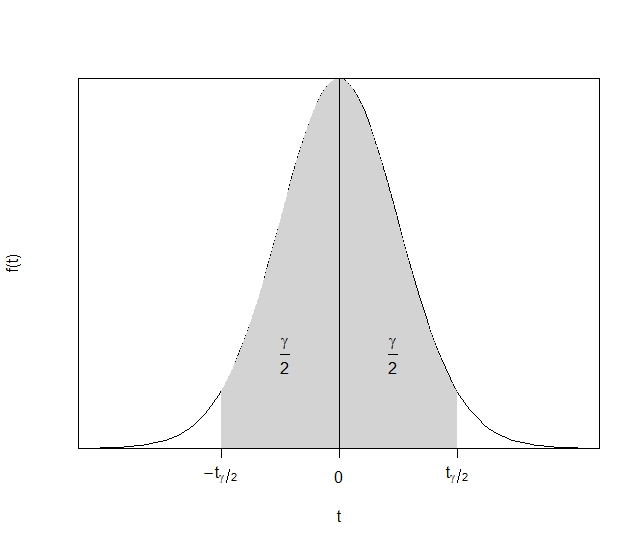
\includegraphics[width=0.5\linewidth]{figs/ICtStudent.jpeg}
	
	\vspace{-0.3cm}
	\small\textit{Distribuição $t$ de Student: mais "espalhada" que a normal, especialmente para amostras pequenas.}
\end{frame}

\begin{frame}{Fórmula do Intervalo de Confiança ($\sigma$ desconhecido)}
	\begin{block}{}
		\justifying
		O intervalo de confiança para $\mu$, quando $\sigma$ é desconhecido, é:
		
		\[
		\left[ \bar{X} - t_{\gamma/2} \cdot \frac{S}{\sqrt{n}} \; ; \;
		\bar{X} + t_{\gamma/2} \cdot \frac{S}{\sqrt{n}} \right]
		\]
		
		\textbf{Interpretação:} Intervalo de valores plausíveis para $\mu$, levando em conta a incerteza tanto da variabilidade amostral quanto da estimativa do desvio padrão.
	\end{block}
\end{frame}
	
	\begin{frame}{Procedimentos para a construção de intervalos de confiança}
		\begin{block}{}
			\justifying
			\begin{enumerate}
				\item Verifique se as suposições necessárias estão satisfeitas
				\begin{itemize}
					\item Temos uma AAS
					\item Temos uma estimativa de $s$
					\item A população tem distribuição normal ou $n>30$
				\end{itemize}
				
				\item Determine o nível de confiança $\gamma$, e encontre o valor crítico $t_{\gamma/2}$
				\item Calcule a margem de erro $e = t_{\gamma/2} \cdot (s/\sqrt{n})$
				\item Calcule $\text{IC}(\mu, \gamma)$
			\end{enumerate}   
		\end{block}
	\end{frame}
	
	\begin{frame}{Exemplo}
		
		\begin{block}{}
			\justifying
			
			Uma turma de Estatística, conhecida por conversar bastante durante as aulas, fez uma prova com nota máxima 100.
			
			Foram selecionadas, aleatoriamente, as notas de \textbf{15 alunos}. A média da amostra foi \textbf{62,4} e o desvio padrão amostral foi \textbf{18,5}.
			
			Segundo relatos, há alguns poucos alunos que prestam muita atenção e puxam as notas para cima, enquanto o resto... conversa.
			
			Construa um intervalo de confiança de 95\% para a média verdadeira das notas dessa turma.
			
		\end{block}
		
	\end{frame}
	
	\begin{frame}{Exemplo}
		
	\small	
		\begin{block}{Solução}
			
			\[
			\bar{X} = 62,4, \quad S = 18,5, \quad n = 15
			\]
			\[
			gl = n - 1 = 14
			\]
			\[
			t_{0,025, 14} = 2,145
			\]
			\[
			e = 2,145 \cdot \frac{18,5}{\sqrt{15}} = 10,24
			\]
			\[
			IC = \left[62,4 - 10,24 \; ; \; 62,4 + 10,24\right]
			\]
			\[
			(52,16 \leq \mu \leq 72,64)
			\]
			
			\textbf{Interpretação:} Com 95\% de confiança, a média real das notas da turma está entre aproximadamente \textbf{52,2 e 72,6}.
			
		\end{block}
		
	\end{frame}
	
	
	
	\section{Intervalo de Confiança para Proporção}
	
	\begin{frame}{Intervalo de Confiança para Proporção}
		\small
		\begin{block}{Distribuição da proporção amostral}
			\justifying
			Seja uma variável aleatória binária com:
			\begin{itemize}
				\item Sucesso: probabilidade $p$;
				\item Fracasso: probabilidade $1-p$.
			\end{itemize}
			
			A proporção amostral é:
			
			\[
			\hat{p} = \frac{x}{n} = \frac{\text{número de sucessos}}{\text{tamanho da amostra}}
			\]
			
			
		\end{block}
	\end{frame}
	
	\begin{frame}{Intervalo de Confiança para Proporção}
		\small
		\begin{block}{}
			
				
			\textbf{Propriedades da distribuição amostral de $\hat{p}$:}
			\begin{itemize}
				\justifying
				\item $\hat{p}$ é um estimador não-viesado de $p$.
				\item Se $n$ é suficientemente grande, $\hat{p}$ segue aproximadamente uma distribuição normal:
				\[
				\hat{p} \sim \text{N} \left( p, \frac{p(1-p)}{n} \right)
				\]
				\item Esperança: $\text{E}(\hat{p}) = p$;
				\item Variância: $\text{Var}(\hat{p}) = \frac{p(1-p)}{n}$.
			\end{itemize}
		\end{block}
	\end{frame}
	
	\begin{frame}{Distribuição amostral da proporção $\hat{p}$}
		\begin{block}{}
			\justifying
			Se a condição de normalidade é satisfeita, podemos padronizar a proporção amostral:
			
			\[
			Z = \frac{\hat{p} - p}{\sqrt{\frac{p(1-p)}{n}}} \sim \text{N}(0,1)
			\]
			
			Isso permite construir intervalos de confiança para $p$ usando a distribuição normal padrão.
		\end{block}
	\end{frame}
	
	\begin{frame}{Fórmula do Intervalo de Confiança}
		\begin{block}{}
			\justifying
			O intervalo de confiança para a proporção populacional $p$, com nível de confiança $\gamma$, é dado por:
			
			\[
			\text{IC}(p, \gamma) =
			\left[
			\hat{p} - z_{\gamma/2} \cdot \sqrt{\frac{\hat{p}(1 - \hat{p})}{n}} \; ; \;
			\hat{p} + z_{\gamma/2} \cdot \sqrt{\frac{\hat{p}(1 - \hat{p})}{n}}
			\right]
			\]
			
			\textbf{Interpretação:} Fornece uma faixa de valores plausíveis para a verdadeira proporção da população.
		\end{block}
	\end{frame}
	
	\begin{frame}{Passos para Construção do Intervalo de Confiança}
		\footnotesize
		\vspace{-0.5cm}
		\begin{block}{}
			\justifying
			\begin{enumerate}
				\item Verifique as suposições:
				\begin{itemize}
					\item A amostra é uma AAS;
					\item As condições da binomial são satisfeitas:
					\begin{itemize}
						\item Tentativas independentes;
						\item Dois resultados possíveis (sucesso/fracasso);
						\item Probabilidade de sucesso constante.
					\end{itemize}
					\item Condição para aproximação normal:
					\[
					n\hat{p} \geq 5 \text{ e } n(1 - \hat{p}) \geq 5
					\]
				\end{itemize}
				
				\item Defina o nível de confiança $\gamma$ e encontre $z_{\gamma/2}$.
				
				\item Calcule a margem de erro e o intervalo:
				\[
				e = z_{\gamma/2} \cdot \sqrt{\frac{\hat{p}(1 - \hat{p})}{n}}\Rightarrow 
				\hat{p} \pm e
				\]
			\end{enumerate}
		\end{block}
	\end{frame}
	
	\begin{frame}{Exemplo - Proporção}
		\begin{block}{}
			\justifying
			Durante uma aula de Estatística, o professor percebe que a turma está mais no WhatsApp do que prestando atenção. Para investigar, ele sorteia uma amostra de 40 alunos e verifica que 28 estavam usando o celular na hora da explicação.
			
			A proporção amostral é:
			
			\[
			\hat{p} = \frac{28}{40} = 0,70
			\]
			
			Construa um intervalo de confiança de 95\% para a proporção de alunos que usam o celular durante a aula.
		\end{block}
		
	\end{frame}
	
	\begin{frame}{Exemplo - Proporção}
		
		\begin{block}{Solução}
			\[
			\hat{p} = 0,70, \; n = 40, \; z_{0,025} = 1,96
			\]
			\[
			e = 1,96 \cdot \sqrt{\frac{0,70 \cdot 0,30}{40}} = 0,144
			\]
			\[
			IC = [0,70 - 0,144 \; ; \; 0,70 + 0,144] = [0,556 \; ; \; 0,844]
			\]
			
			\textbf{Interpretação:} Com 95\% de confiança, entre 55,6\% e 84,4\% dos alunos usam o celular durante a aula.
		\end{block}
	\end{frame}
	
	\section{Determinação do Tamanho Amostral ($\sigma$ conhecido)}
	
	\begin{frame}{Determinação do Tamanho Amostral}
		\begin{block}{}
			\justifying
			Nosso objetivo é coletar dados para estimar a \textbf{média populacional} $\mu$.
			
			A grande pergunta é:
			
			\begin{center}
				\textbf{Quantos elementos (pessoas, objetos, itens...) devemos amostrar?}
			\end{center}
			
			Sabemos que, de forma geral, $n > 30$ costuma ser suficiente para muitas situações.
			
			Mas... podemos ser mais inteligentes que isso! 
			
			\textbf{Existe uma fórmula que permite calcular exatamente o tamanho de amostra necessário, baseado na precisão desejada.}
		\end{block}
	\end{frame}
	
	\begin{frame}{Fórmula para o Tamanho Amostral}
		\begin{block}{Derivação}
			Sabemos que a \textbf{margem de erro} para a média é dada por:
			
			\[
			e = z_{\gamma/2} \cdot \frac{\sigma}{\sqrt{n}}
			\]
			
			Isolando $n$:
			
			\[
			n = \left( \frac{z_{\gamma/2} \cdot \sigma}{e} \right)^2
			\]
			
			\textbf{Esta é a fórmula que usamos para calcular o tamanho amostral necessário.}
		\end{block}
	\end{frame}
	
	\begin{frame}{Interpretando a Fórmula}
		\begin{block}{O que influencia o tamanho amostral?}
			
			\[
			n = \left( \frac{z_{\gamma/2} \cdot \sigma}{e} \right)^2
			\]
			
			\textbf{O tamanho amostral depende de:}
			\begin{itemize}
				\item O \textbf{nível de confiança} desejado ($z_{\gamma/2}$);
				\item O \textbf{erro máximo admissível} ($e$) \textendash{} \textit{precisão desejada};
				\item O \textbf{desvio padrão populacional} ($\sigma$).
			\end{itemize}
			
			\textbf{Não depende} do tamanho da população (se for muito grande).
			
			\textbf{Importante:} Sempre arredondamos $n$ para o \textbf{próximo número inteiro superior}.
		\end{block}
	\end{frame}
	
	\begin{frame}{Exemplo - Determinação do Tamanho Amostral}
		\begin{block}{}
			\justifying
			Queremos estimar o tempo médio que alunos passam no WhatsApp por semana.
			
			Desejamos um intervalo de confiança de 95\%, com \textbf{margem de erro de no máximo 2 horas}. Estudos anteriores indicam que o desvio padrão é \textbf{5,2 horas}.
			
			Qual deve ser o tamanho da amostra?
		\end{block}
	
	\end{frame}
	
	\begin{frame}{Exemplo - Determinação do Tamanho Amostral}

		\begin{block}{Solução}
			\[
			\sigma = 5,2, \; e = 2, \; z_{0,025} = 1,96
			\]
			\[
			n = \left( \frac{1,96 \cdot 5,2}{2} \right)^2 = \left(5,096\right)^2 = 25,97
			\]
			\[
			n = 26 \text{ (arredondado para o inteiro superior)}
			\]
			
			\textbf{Conclusão:} Precisamos de uma amostra com pelo menos 26 alunos.
		\end{block}
	\end{frame}
	

	
\section{Determinação do Tamanho Amostral ($\sigma$ desconhecido)}

\begin{frame}{Determinação do Tamanho Amostral ($\sigma$ desconhecido)}
	\vspace{-0.5cm}
	\small
	\begin{block}{}
		\justifying
		Se \(\sigma\) for desconhecido, temos algumas estratégias práticas:
			\vspace{-0.3cm}
		\begin{itemize}
			\justifying
			\item Utilizar uma \textbf{estimativa de $\sigma$} baseada em estudos anteriores ou literatura;
			\item Realizar uma \textbf{amostra piloto} e utilizar o desvio padrão amostral ($s$) como aproximação de $\sigma$;
			\item Usar a \textbf{regra empírica da amplitude}, válida para dados aproximadamente normais:
			\[
			\sigma \approx \frac{\text{amplitude}}{4}
			\]
			onde amplitude é \(\max - \min\) de valores típicos (sem outliers extremos).
		\end{itemize}
		
	\end{block}
\end{frame}

\begin{frame}{Regra Empírica para Estimar $\sigma$}
	\centering
	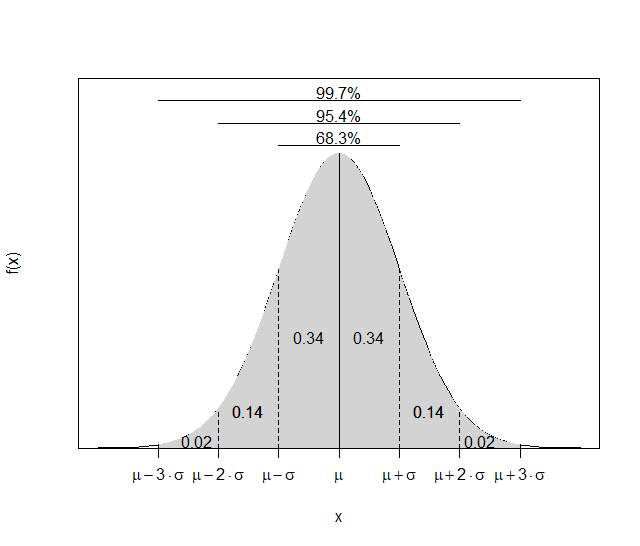
\includegraphics[width=0.7\linewidth]{figs/ICEmpirico.png}
	
	\vspace{0.3cm}
	\small\textit{Aproximadamente 95\% dos dados de uma distribuição normal estão entre \(\mu - 2\sigma\) e \(\mu + 2\sigma\).}
\end{frame}

\begin{frame}{Aplicando a Regra Empírica}
	\vspace{-0.5cm}
		\small
	\begin{block}{}
		\justifying
		Definimos como \textbf{valores usuais} aqueles que não são extremos.
		
		Para uma distribuição aproximadamente normal, sabemos que:
		
		\[
		4\sigma \approx \text{amplitude} = \max - \min
		\]
		
		Portanto, uma estimativa prática para \(\sigma\) é:
		
		\[
		\sigma \approx \frac{\max - \min}{4}
		\]
		
		Essa técnica é muito útil quando não temos dados prévios ou quando queremos uma estimativa rápida e prática.
	\end{block}
\end{frame}
	
	\begin{frame}{Exemplo - Determinação do Tamanho Amostral}
		
		\begin{block}{}
			\justifying
			Uma clínica deseja estimar o \textbf{tempo médio de espera dos pacientes para atendimento}.
			
			Eles querem garantir que a média amostral esteja, no máximo, \textbf{5 minutos distante da média real}, com \textbf{90\% de confiança}.
			
			Sabe-se que os tempos de espera costumam variar entre \textbf{10 e 50 minutos}.
			
			\textbf{Pergunta:} Qual deve ser o tamanho da amostra?
			
		\end{block}
		
	\end{frame}
	
	\begin{frame}{Exemplo - Determinação do Tamanho Amostral}
		\vspace{-0.5cm}
		\small
		\begin{block}{}
			
			Estimando o desvio padrão usando a regra empírica:
			
			\[
			\sigma = \frac{50 - 10}{4} = 10
			\]
			
			Para 90\% de confiança, \(z_{0,05} = 1,645\).
			
			Aplicando a fórmula:
			
			\[
			n = \left( \frac{1,645 \cdot 10}{5} \right)^2 = (3,29)^2 = 10,82
			\]
			\[
			n = 11 \text{ (arredondado para o inteiro superior)}
			\]
			
			\textbf{Conclusão:} É necessário amostrar pelo menos 11 pacientes para estimar a média do tempo de espera com a precisão desejada.
			
		\end{block}
		\nocite{Morettin09, Apostila, eric, montgomery2016, meyer1982probabilidade, Bastos2025}
	\end{frame}
	
	
	
	%\begin{frame}{Exemplo - Determinação do Tamanho Amostral}
	%
	%\begin{block}{}
	%\justifying
	%Um professor deseja estimar o \textbf{tempo médio que seus alunos passam no WhatsApp por semana}.
	%
	%Ele quer garantir que a média amostral esteja, no máximo, \textbf{2 horas distante da média real}, com \textbf{90\% de confiança}.
	%
	%Sabe-se que, segundo levantamentos informais, os tempos variam entre \textbf{10 horas e 30 horas por semana}.
	%
	%\textbf{Pergunta:} Qual deve ser o tamanho da amostra?
	%        
	%        \end{block}
	%
	%\pause
	%
	%\begin{block}{Solução}
	%
	%Estimando o desvio padrão usando a regra empírica:
	%        
	%        \[
	%                \sigma = \frac{30 - 10}{4} = 5
	%                \]
	%
	%Para 90\% de confiança, \(z_{0,05} = 1,645\).
	%
	%Usando a fórmula:
	%        
	%        \[
	%                n = \left( \frac{1,645 \cdot 5}{2} \right)^2 = \left(4,1125\right)^2 = 16,92
	%                \]
	%\[
	%        n = 17 \text{ (arredondado para o inteiro superior)}
	%        \]
	%
	%\textbf{Conclusão:} É necessário amostrar pelo menos 17 alunos.
	%
	%\end{block}
	%
	%\end{frame}
	%
	%
	%\begin{frame}{}
	%\begin{block}{Exemplo}
	%\justifying
	%Um professor deseja estimar o salário médio de professores do Ensino Médio de uma cidade. Quantos professores devem ser selecionados para termos 90\% de confiança que a média amostral esteja a menos de R\$30,00 da média populacional? Sabe-se apenas que os
	%salários variam entre R\$800,00 e R\$1.200,00. Use
	%$$
	%        n = \left[ \frac{z_{\gamma/2} \cdot \sigma}{e} \right]^2
	%$$  
	%        \nocite{Apostila}
	%%\begin{verbatim}
	%%zcrit <- qnorm(0.95)
	%%erro <- 30
	%%sigma <- (1200 - 800)/4
	%%((zcrit * sigma)/erro)^2    
	%%\end{verbatim}
	%\end{block}
	%
	%\end{frame}
	
	\begin{frame}[allowframebreaks]
		\frametitle{\bf Referências}
		\printbibliography
	\end{frame}
	
	
\end{document}
